\documentclass[10pt]{article}
\usepackage[utf8]{inputenc}
\usepackage[T1]{fontenc}
\usepackage{amsmath}
\usepackage{amsfonts}
\usepackage{amssymb}
\usepackage{stmaryrd}
\usepackage{hyperref}
\hypersetup{colorlinks=true, linkcolor=blue, filecolor=magenta, urlcolor=cyan,}
\urlstyle{same}
\usepackage{graphicx}
\usepackage[export]{adjustbox}
\usepackage{mdframed}
\usepackage{booktabs,array,multirow}
\usepackage{esint}
\usepackage{xeCJK}
\usepackage{adjustbox}
\newcommand{\HRule}{\begin{center}\rule{0.5\linewidth}{0.2mm}\end{center}}
\graphicspath{ {./images/} }
\begin{document}

\section*{【知识模块 3】膜电池}

膜的引入简化了装置, 用离子交换膜分隔成两池, 仅允许特定的离子通过; 且膜能持续、长期使用。

\begin{center}
\includegraphics[max width=0.9\textwidth]{images/0190d991-935a-7a64-a143-43f70f75daa5_0_602874.jpg}
\end{center}

膜的分类: 叫他就只让他离子过

①阳离子交换膜

②阴离子交换膜

③质子交换膜

\[
\text{只有}{\mathrm{H}}^{ + }\text{能过}
\]

④双极膜

\[
{H}_{2}O \rightleftharpoons {H}^{2} + O{H}^{ - } - 1\text{ 或者 } - 2\text{ 或 } - 2
\]

\section*{【经典】}

1.【2020 嘉兴期末】某硫酸厂运用电化学原理设计了如图所示的装置,实现了在用 \({\mathrm{{SO}}}_{2}\) 发电的同时制备硫酸。图中电极是含催化剂、多孔吸附性的惰性材料。下列说法正确的是 ( \(D\) )

\begin{center}
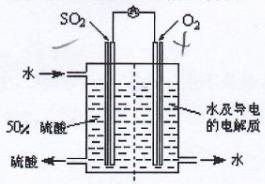
\includegraphics[max width=0.3\textwidth]{images/0190d991-935a-7a64-a143-43f70f75daa5_0_718268.jpg}
\end{center}

质子膜

(只允许H*通过

A. \({\mathrm{{SO}}}_{2}\) 气体在电极表面得电子,生成硫酸

B. 该装置工作时的总反应: \(2{\mathrm{{SO}}}_{2} + {\mathrm{O}}_{2} + 2{\mathrm{H}}_{2}\mathrm{O} = 2{\mathrm{H}}_{2}{\mathrm{{SO}}}_{4}\) .

C. 正极的电极反应: \({\mathrm{O}}_{2} + 4\mathrm{e} = 2{\mathrm{O}}^{2 - }\)

D. 氢离子向负极区移动,与负极生成的 \({\mathrm{{SO}}}_{4}{}^{2 - }\) ,结合形成硫酸而被排出

\end{document}